\documentclass[a4paper,11pt]{article}
\usepackage[margin=25mm]{geometry}
\usepackage[T1]{fontenc}
\usepackage[utf8]{inputenc}
\usepackage{amsmath,amssymb,booktabs,array}
\usepackage{graphicx,microtype,placeins,setspace}
\usepackage[font=small,labelfont=bf]{caption}
\usepackage[colorlinks=true,allcolors=blue,pdfauthor={}]{hyperref}
\onehalfspacing
\pagestyle{plain}
\newcommand{\gd}{\ensuremath{\gamma\delta}}
\newcommand{\gtd}{\mbox{\ensuremath{\gamma\!\rightarrow\!\delta}}}
\newcommand{\dtg}{\mbox{\ensuremath{\delta\!\rightarrow\!\gamma}}}
\title{Benchmarking single-CDR3 recorded-partner recovery in human gamma-delta T-cell receptors under controlled exposure protocols}
\author{}
\date{}
\begin{document}
\maketitle
\begin{abstract}
\textbf{Background:} Single-chain receptor models can generate plausible
complementarity-determining region 3 (CDR3) sequences without recovering the
partner recorded for an input chain. Evaluation must distinguish target-sequence
priors, conditional information, candidate availability and exposure to related
sequences. We assembled 9068 unique human gamma-delta T-cell receptor CDR3
pairs and compared a denoising-pretrained conditional Transformer with matched
constant-source, random-initialization and shuffled-input controls. The primary
endpoint was equal-direction mean query-macro Hit@5 at 64 draws under
component-disjoint splitting. Free generation, truth-containing fixed-pool
retrieval and additional exposure protocols were evaluated separately, with
pair ranking as a secondary component.

\textbf{Results:} Mean target-token negative log likelihood was 1.005 nats for
the pretrained conditional model, 1.013 for the constant-source prior and 1.115
for random initialization. Primary free-generation likelihood Hit@5 was
0.03\%; ranker Hit@5 was 0.06\%, without a reproducible improvement across
fitted comparisons. Fixed-pool retrieval was easier than free generation and
depended on direction and distractor construction. Nearest-input
partner-similarity ranking was competitive in some gamma-to-delta pools.
Higher recovery under some target-exposed and source-specific protocols
coexisted with substantial prior-model recovery and clustered events.
Training-size comparisons also changed graph composition, while additional
sampling increased coverage without ensuring top-five recovery.

\textbf{Conclusions:} Denoising pretraining improved target-token likelihood,
but the conditional contribution beyond a matched target prior was modest and
free recorded-partner recovery remained sparse. Separately trained reranking
showed no reproducible primary benefit. These results support explicit
separation of sequence modeling, candidate availability, ranking and exposure
when evaluating single-CDR3 partner recovery. They do not establish biological
function, a mechanism of pairing or transfer to distant sequences.
\end{abstract}

\noindent\textbf{Keywords:} gamma-delta T cells; T-cell receptor pairing; CDR3;
conditional generation; benchmarking

\section{Background}
Gamma-delta T-cell receptors (\gd{} TCRs) are heterodimers whose biological
interpretation depends on both chains and on the surrounding receptor and
cellular context \cite{gd_review}. Sequence databases make it possible to learn
chain-specific regularities from many unpaired receptors, whereas paired
observations provide a smaller and less complete description of which chains
occur together. Predicting a recorded partner from a single CDR3 is therefore
a distinct problem from generating a plausible receptor-like sequence.
The target chain may be plausible under a sequence prior without carrying
information specific to the input. Establishing that distinction is necessary
before using conditional scores to prioritize candidates for further study.

Public resources support several related computational tasks. UcTCRdb and
TCRdb 2.0 provide unconventional or gamma/delta repertoires
\cite{uctcrdb,tcrdb2}, and the Observed T Cell Receptor Space database enables
paired-chain analysis and conditional residue infilling \cite{ots}.
TCR-BERT explores self-supervised representations \cite{tcrbert}, whereas
TCRBinder and TCRdesign address peptide recognition using paired alpha/beta
inputs or antigen-conditioned beta-CDR3 design \cite{tcrbinder,tcrdesign}.
These advances motivate sequence modeling but do not supply directly
transferable performance baselines for gamma/delta partner recovery.
Pretraining loss can itself be a poor proxy for downstream benefit
\cite{landry2025}; improved reconstruction must consequently be distinguished
from improved recovery of a recorded paired chain.

Pairing studies in alpha/beta receptors have identified inter-chain sequence
constraints \cite{pairing_constraints}. TCRpair predicts functional pairing
in an HLA-A*02:01-restricted alpha/beta setting and includes residues flanking
CDR3 \cite{tcrpair}. Epitope-conditioned diffusion models address another
generation task \cite{dtcr}. Their inputs, populations and endpoints differ
from the single-CDR3 gamma/delta problem considered here. A recent
immune-receptor retrieval preprint also motivates attention to sequence
alignment baselines and clonal exposure \cite{germline_shortcut}.
Local sequence similarity may support ranking even when a model has not
learned an input-specific rule that transfers to a previously unseen chain.
Structure-based specificity prediction using AlphaFold 3 likewise evaluates
MHC:peptide:TCR recognition rather than gamma/delta chain completion
\cite{af3_specificity}.

Three evaluation distinctions are particularly relevant. First, a matched
target-prior control is needed to separate conditional information from the
distribution of frequent or easy-to-model targets. Second, ranking a fixed
pool that contains a recorded positive does not test whether a free generator
can produce that positive. Third, exact sequence separation does not remove
near-neighbor exposure, and withholding an edge between known chains differs
from withholding a complete pairing-graph component. These distinctions
affect the interpretation of both positive and negative results.

The evaluation unit also matters when one input has several recorded
partners. Weighting every pair equally emphasizes highly connected inputs,
whereas weighting queries equally asks how often an input is served by the
model. A benchmark should make this choice explicit and preserve it across
controls. In the present study, the primary query-macro endpoint treats input
queries equally within each direction, then gives the two directions equal
weight. Graph components provide the resampling unit for the primary paired
comparison because their edges share receptor chains.

The model sees neither full receptor sequence nor V/J genes, antigen identity
or structural context. A successful benchmark outcome would therefore concern
recorded CDR3 pairing under restricted inputs. Conversely, a missed database
partner need not be a functionally incompatible sequence. Keeping the input
scope and observation process explicit makes the benchmark interpretable
alongside richer pairing and specificity tasks.

Here we ask whether denoising pretraining improves partner modeling relative
to random initialization, whether the input chain improves recovery beyond a
matched target prior, and whether separate pairwise ranking improves candidate
ordering. We evaluate these questions under explicit exposure protocols,
retain multiple recorded partners per input, and compare models using shared
test queries and saved candidates. The contribution is a controlled benchmark
with interpretable controls and uncertainty units. Its conclusions concern the
tested model family, training settings and recorded data; they do not establish
that partner prediction is intrinsically impossible or that generated receptors
have biological function.

\section{Methods}
\subsection{Data assembly and preprocessing}
The paired corpus contains 9068 unique CDR3 pairs: 8443 traced to GSE180059
\cite{gse180059}, 626 to Suo et al.\ through UcTCRdb \cite{suo2022,uctcrdb},
and one IEDB-export pair with unresolved original-study provenance \cite{iedb}.
Two pairs occur in both major sources. GSE180059 profiles fetal and pediatric
thymocytes, and Suo et al.\ profile the developing prenatal immune system.
These are publicly recorded pairings rather than complete biological ground
truth, and they do not represent the full adult peripheral repertoire.
Extended methods and source audits are supplied in Additional files 1 and 2.

Cleaning uppercases and exact-deduplicates canonical amino-acid sequences,
retaining source-provided CDR3 boundaries. GEO contigs must satisfy cell,
productive, high-confidence and full-length flags; a library-local barcode is
paired only when one distinct accepted gamma and one delta CDR3 remain.
Equivalent cell-quality information is unavailable for some exports.
Observation-level records retain source membership, library-local barcodes and
available V/J annotations. The models use only CDR3. Donor identity cannot be
fully recovered, so no evaluation is designated donor-independent.

Single-chain inputs contain 194887 gamma and 1262692 delta sequences before
pretraining filters. All paired-corpus chains and sequences shorter than six
residues are excluded. The main pretraining pool has 187092 gamma and 1230589
delta training sequences, with 3818 and 25114 validation sequences.
The two source protocols use the same additional study-excluded pretraining
pool. Training and validation are disjoint at the unique-sequence level.
Pool sizes, seeds, selected checkpoints and actual exposure are detailed in
Additional files 1 and 3.

\subsection{Exposure protocols and data partitions}
Unique gamma and delta CDR3s form the two node sets of a bipartite graph, with
recorded pairs as edges. Whole components define primary splits with seeds
17, 3407 and 2026, each containing 7254/907/907 training/validation/test edges.
Neither chain overlaps exactly across these partitions. The largest component
is assigned wholly to training. Allocation targets edge counts without
optimizing source or length balance.

Primary validation components are divided into checkpoint selection, tuning
and calibration roles with 453/227/227 edges using seed 7319. Directional
protocols instead preserve input-query groups. No test result selects a
checkpoint, fusion weight, sampling rule or threshold. The primary analysis
protocol was specified after earlier exploratory results had been examined;
it was not preregistered. Those earlier estimates used different selection
and validity rules and are excluded from the primary summaries.

Unseen-input diagnostics withhold gamma or delta queries while allowing target
overlap. Seen-input diagnostics withhold edges from inputs with at least three
partners while retaining a training edge for each input. Strict study holdout
excludes traceable held-study chains from supervised training; source-shared
evaluation retains common chains. Both test the same 626 Suo pairs, but their
training sizes and exposure differ. They assess study-level sensitivity,
without a donor-independent prospective validation claim.

Two further diagnostics examine evaluation design. The original unseen-gamma
selection set contained one query, 581 targets and no ranking distractors.
Reallocation by whole query groups gives 31/16/16 selection/tuning/calibration
queries while preserving training, aggregate validation and test membership.
The resulting refits use two seeds and fixed 64-draw evaluation.
Within the giant component, 1000 edges are reserved while both endpoints
retain training edges, then divided into 500 validation and 500 test edges.
The remaining training set has 6254 edges. All held-out endpoints are exposed
and all test edges originate from one component; this diagnostic therefore
reports counts and point estimates without an inferential component interval.
Reservation rules and historical estimates are retained in Additional file 1.

The query-balanced unseen-gamma selection set contains 275 edges and at least
118 eligible distractors per query. Its tuning and calibration roles are
retained but do not select new settings for the refits. Within-component
reservation and assignment use seeds 1729 and 1730; all 500 validation edges
select checkpoints, with no subsequent fusion or threshold tuning.
These analyses address identified design limitations while preserving the
primary test. Their estimates are not pooled with the primary population.

\subsection{Conditional generator and matched controls}
The shared encoder--decoder Transformer has 7396890 parameters, four encoder
and four decoder layers, width 256, eight attention heads, feedforward width
1024 and dropout 0.1. Amino-acid and chain-control tokens represent inputs up
to 64 tokens. The model learns both $p_\theta(d\mid g)$ and
$p_\theta(g\mid d)$. Teacher-forced target-token negative log likelihood (NLL)
includes end of sequence (EOS) and excludes padding and chain-control
prediction.

Denoising uses 20000 steps, batch size 1024 and AdamW at
$3\times10^{-4}$, with 500 warmup steps. Masking rates of 15\% and 30\%
are equally likely; selected sites undergo mask/random/unchanged replacement
at 80/10/10 proportions, followed by short-span deletions targeting
approximately 8\% of positions. Reconstruction is evaluated on frozen
corruptions, including selected-but-unchanged sites, against an aligned-copy
control. The square-root chain mixture is primary; other mixtures and their
actual sequence/token exposures are sensitivities in Additional file 1.

Paired fine-tuning uses at most 1500 steps, batch size 256, learning rate
$2\times10^{-5}$, 200 warmup steps, validation every 100 steps and patience
five. Sampling chooses directions equally, input queries uniformly and one
recorded partner uniformly within each query. Selection uses query-macro
partner NLL. The constant-source control removes input residues while
matching initialization, target sampling and optimization. Random initialization
matches downstream settings but omits pretraining; total computation is not
matched. Shuffled-input evaluation permutes queries of the fitted conditional
model without retaining their partner association.

The pair ranker is a secondary evaluation of candidate ordering.
It initializes from a separate copy of the selected generator's encoder and
trains that encoder and a scoring head on the same training edges, leaving
the source generator fixed. Training uses multi-positive contrastive loss
followed by equally weighted positive and constructed-negative binary
cross-entropy. Negatives are unrecorded combinations, not verified biological
incompatibilities. Architecture, optimization, negative sampling and checkpoint
selection are fully specified in Additional file 1.
Figure~\ref{fig:workflow} summarizes the model and evaluation workflow.

Training-size sensitivities use nested complete-component subsets and the
same pretrained and random-initialization conditions. Edge-uniform sampling
is a separate control for the query-uniform training objective.
Unidirectional sensitivity models receive at most 750 steps and 100 warmup
steps to match nominal per-direction sequence exposure; directional exposure
diagnostics retain the 1500-step maximum. Actual early-stopping exposure is
reported independently of these nominal budgets. These controls evaluate
specific design choices and are not additional methods selected for favorable
test performance.

\begin{figure}[!htbp]
\centering
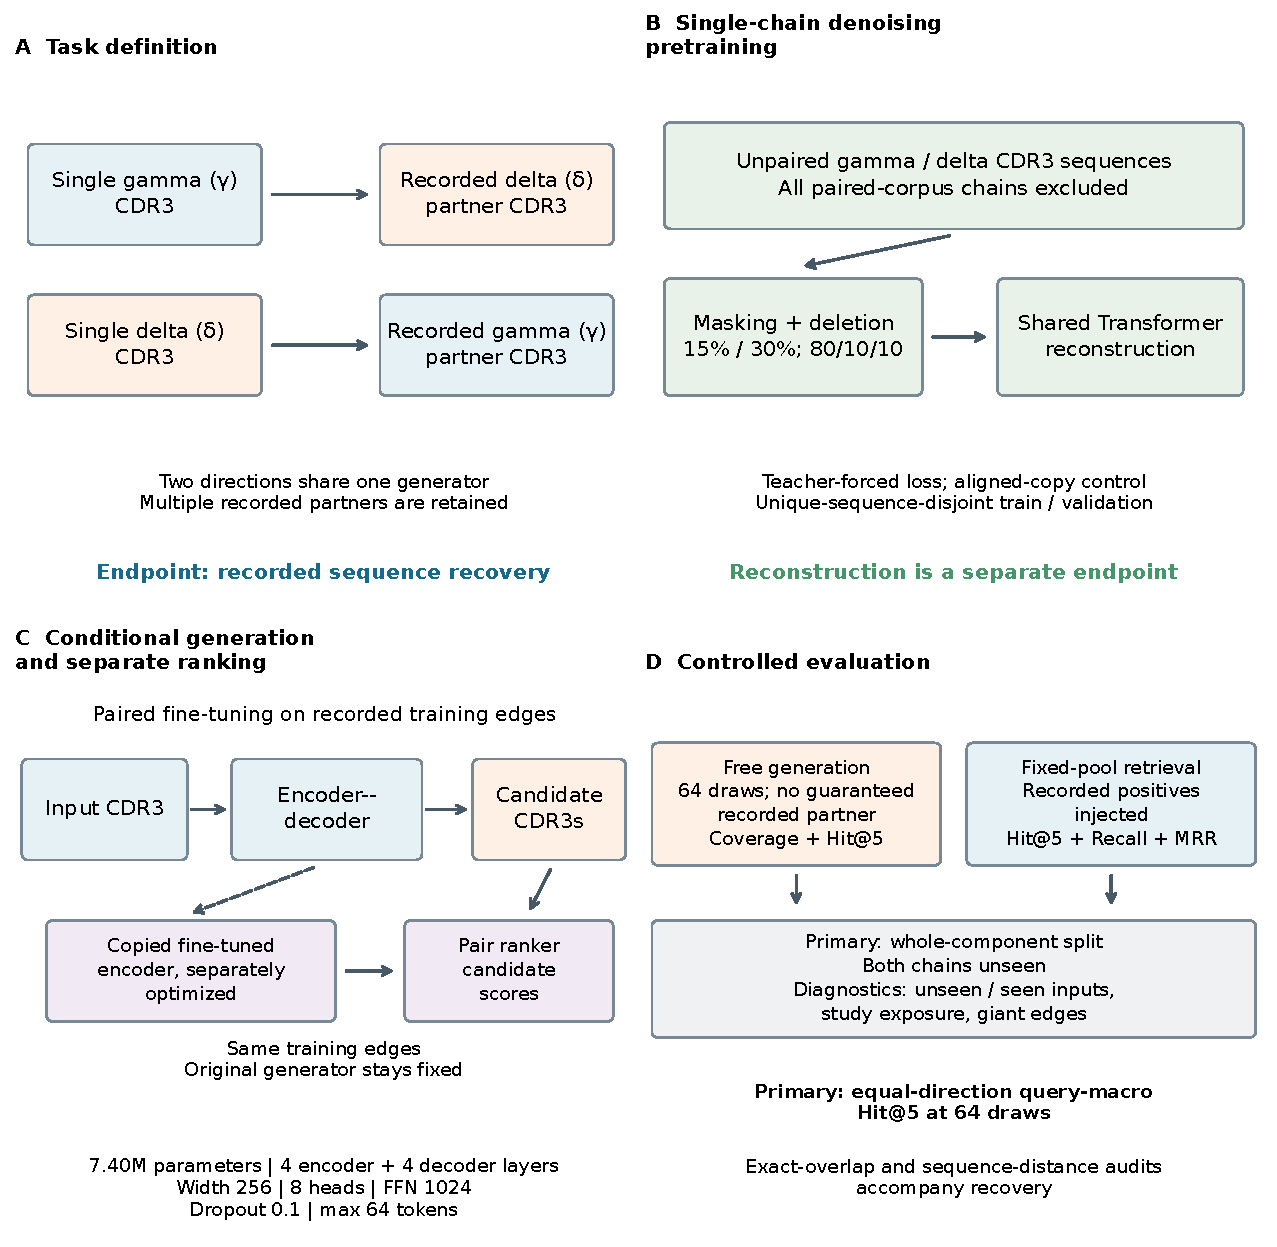
\includegraphics[width=\linewidth]{../results/bmc/figures/figure_1_workflow.pdf}
\caption{Overview of the single-CDR3 partner-recovery benchmark and model workflow. A: each task maps one gamma or delta CDR3 to recorded partner CDR3s. B: denoising pretraining excludes all paired-corpus chains. C: conditional generation and separately trained ranking share training-edge and encoder provenance. The ranker optimizes its copied encoder; the original generator remains fixed. D: free generation and truth-containing retrieval are different endpoints. The primary endpoint is equal-direction mean query-macro Hit@5 at 64 draws under component-disjoint splitting; other exposure protocols are diagnostics.}
\label{fig:workflow}
\end{figure}
\FloatBarrier

\subsection{Free generation and fixed-pool retrieval}
Primary free generation uses 64 draws at temperature one and top-$p=0.95$.
Validity requires 6--35 canonical residues and observed EOS, allowing 36
decoding steps. Invalid or duplicate draws are not replaced. Training targets
are allowed in the primary analysis; exact training-target exclusion is a
separate policy that can remove legitimate positives in exposed-target tasks.
Free generation never injects a recorded test partner into the candidate set.

Fixed pools contain all role-specific recorded positives and up to 100
unrecorded targets selected by random, length, terminal-motif or edit matching.
Full retrieval uses the complete role-specific target universe.
Other recorded partners are excluded from distractors; all scorers and seeds
share frozen candidate lists. Score ties use lexicographic sequence order.
These pools explicitly measure ranking when positives are available.

Scorers include conditional and prior likelihood, shuffled-input likelihood,
their conditional-minus-prior difference, ranker, fused and seeded random
scores. Likelihood is negative per-target-token NLL including EOS, so its
difference is a length-normalized log score. Training-target frequency,
shallow length/terminal features and a two-chain edit-neighbor score provide
additional references. Nearest-input direct transfer proposes recorded
training partners of one or five nearest inputs, with deterministic distance
ties and at most 64 unique targets. A separate partner-similarity score ranks
supplied pool candidates by distance to partners of the nearest training
input. This extension can score a withheld target without proposing it.
Construction details and sensitivities are in Additional file 1.

Direct-transfer targets are ordered by descending training degree and then
lexicographically, with the five-neighbor sensitivity concatenating these
lists in neighbor order. The nearest input is selected using normalized
full-CDR3 Levenshtein distance and lexicographic ties. Partner-similarity
ranking uses minimum normalized target distance to that input's known
training partners. The separate two-chain neighbor score minimizes average
normalized gamma and delta distances jointly over every training edge.
These definitions distinguish copying observed partners from scoring a
candidate universe that includes previously withheld sequences.

Direction-specific score standardization and fusion weights are selected on
tuning data, with ties favoring less ranker weight. An independent calibration
role selects acceptance thresholds; missing either label class yields
reject-all. These thresholds distinguish recorded positives from constructed
combinations, not biological binding. Sampling-budget, decoding-grid and
calibration analyses are secondary and retain the primary setting unchanged.

\subsection{Endpoints and statistical analysis}
For input query $q$, let $P_q$ be its recorded test partners, $C_q$ its unique
valid candidates and $C_q^{(K)}$ its first $K$ ranked candidates. We define
\begin{equation}
\mathrm{Coverage}(q)=\mathbf{1}(P_q\cap C_q\ne\varnothing),\qquad
H_K(q)=\mathbf{1}(P_q\cap C_q^{(K)}\ne\varnothing).
\end{equation}
The primary endpoint equally averages directional query-macro Hit@5 at 64
draws. Likelihood, ranker and fused ordering use identical generator candidates.
Coverage tests candidate availability; Hit@5 also tests their ordering.
Per-fit events and query outcomes appear in Additional file 4; split
assignments, fixed pools and free-candidate hashes appear in Additional file 5.
Recall, reciprocal rank, token-weighted NLL, validity, uniqueness, novelty and
diversity are secondary summaries defined in Additional file 1.

For target $y$, let $T_y=|y|+1$, with EOS at position $T_y$. Query-macro NLL
averages target tokens within partner, partners within query and queries within
direction:
\begin{align}
\ell(q,y)&=-\frac{1}{T_y}\sum_{i=1}^{T_y}\log p_\theta(y_i\mid q,y_{<i}),\\
L_d&=\frac{1}{|Q_d|}\sum_{q\in Q_d}\frac{1}{|P_q|}
 \sum_{y\in P_q}\ell(q,y),\qquad
L_{\rm macro}=\frac{L_{\gamma\rightarrow\delta}+L_{\delta\rightarrow\gamma}}{2}.
\end{align}
Partners and queries receive equal weight at their respective levels;
longer targets receive no additional weight. Checkpoint selection uses the
same hierarchy, restricted to one direction for directional fits.
Token-weighted reporting divides summed losses by total target tokens.
The optimization loss averages non-ignored tokens within each minibatch,
which differs from the query-macro reporting hierarchy.

Paired uncertainty uses 2000 bootstrap resamples of complete test components,
or input-query groups for directional diagnostics. Joint directional
comparisons share component resamples and retain equal directional weighting.
Comparisons align queries, positives and cluster identities, and use identical
candidate pools where relevant. Two model seeds are averaged within each
primary split before calculating the mean and sample standard deviation (SD)
of the three split means. These SDs are descriptive, not confidence intervals.
Repeated splits and seeds are not independent biological replicates.
Bootstrap intervals condition on fitted models and saved candidates, without
multiplicity adjustment; a zero-event $[0,0]$ interval is not a population
upper bound.

Sequence exposure is assessed by minimum Levenshtein distance to supervised
and pretraining references. A distant edge requires both input and eligible
recorded target to be at least three edits from both pools. Source, length,
partner multiplicity and component-size strata retain original query labels,
candidates and clusters and are descriptive. AUC summaries report positive
prevalence, recognizing the limitations of imbalanced classification
\cite{pr_metrics}.

\subsection{Computational environment and reproducibility}
The environment uses Python 3.10.20, PyTorch 2.7.1 and CUDA 12.6.
Primary fitting used A800 GPUs and the additional exposure fits used RTX 3090
GPUs; no controlled hardware-performance comparison is inferred.
Frozen source snapshots and input/output hashes link configurations,
checkpoints, candidates and analyses. Actual training exposure is recorded
alongside nominal budgets. Additional file 6 provides source, configuration
and environment records, and the public repository provides a portable
reproduction workflow. Reproducing training on different hardware need not
yield byte-identical weights.

\section{Results}
\subsection{Dataset structure and sequence exposure}
The 9068 pairs contain 3944 gamma and 6989 delta CDR3s, distributed across
3294 components, including 2897 single-edge components. The largest component
contains 5005 edges (55.2\%) and remains wholly in training. Maximum gamma
and delta degrees are 581 and 140; 767 gamma and 519 delta nodes have multiple
recorded partners. Thus, a CDR3 does not have a unique pairing label.
GSE180059 contributes 93.1\% of the paired union, limiting supervision diversity
(Table~\ref{tab:data}).

\begin{table}[!htbp]
\centering
\caption{Primary split structure and proximity to the pretraining pool. Distance bins use unique test gamma queries; these are not donor-level external tests. Distant edges require both chains to be at least three edits from supervised and pretraining references.}
\label{tab:data}
\small
\setlength{\tabcolsep}{3pt}
\begin{tabular}{>{\raggedright\arraybackslash}p{0.4200\linewidth}p{0.1600\linewidth}p{0.1600\linewidth}p{0.1600\linewidth}}
\toprule
Split seed & 17 & 3407 & 2026\\
\midrule
Training/validation/test edges & 7254/907/907 & 7254/907/907 & 7254/907/907\\
Test gamma queries & 529 & 523 & 525\\
Test delta queries & 900 & 906 & 904\\
Gamma queries one edit from pretraining & 487 & 494 & 493\\
Gamma queries at least three edits from pretraining & 8 & 7 & 4\\
Distant test edges & 5 & 5 & 3\\
Largest-component assignment & Training & Training & Training\\
\bottomrule
\end{tabular}
\end{table}
\FloatBarrier

Exact chain separation does not eliminate near-neighbor exposure.
Across the three primary tests, 487/529, 494/523 and 493/525 gamma queries
are one edit from a pretraining sequence. Requiring both chains to be at
least three edits from both reference pools leaves only 5, 5 and 3 test
edges. Neither source test has an edge satisfying this condition.
The graph and sequence landscape therefore restricts what the primary
benchmark can establish about distant-sequence transfer (Figure~\ref{fig:data}).

\begin{figure}[!htbp]
\centering
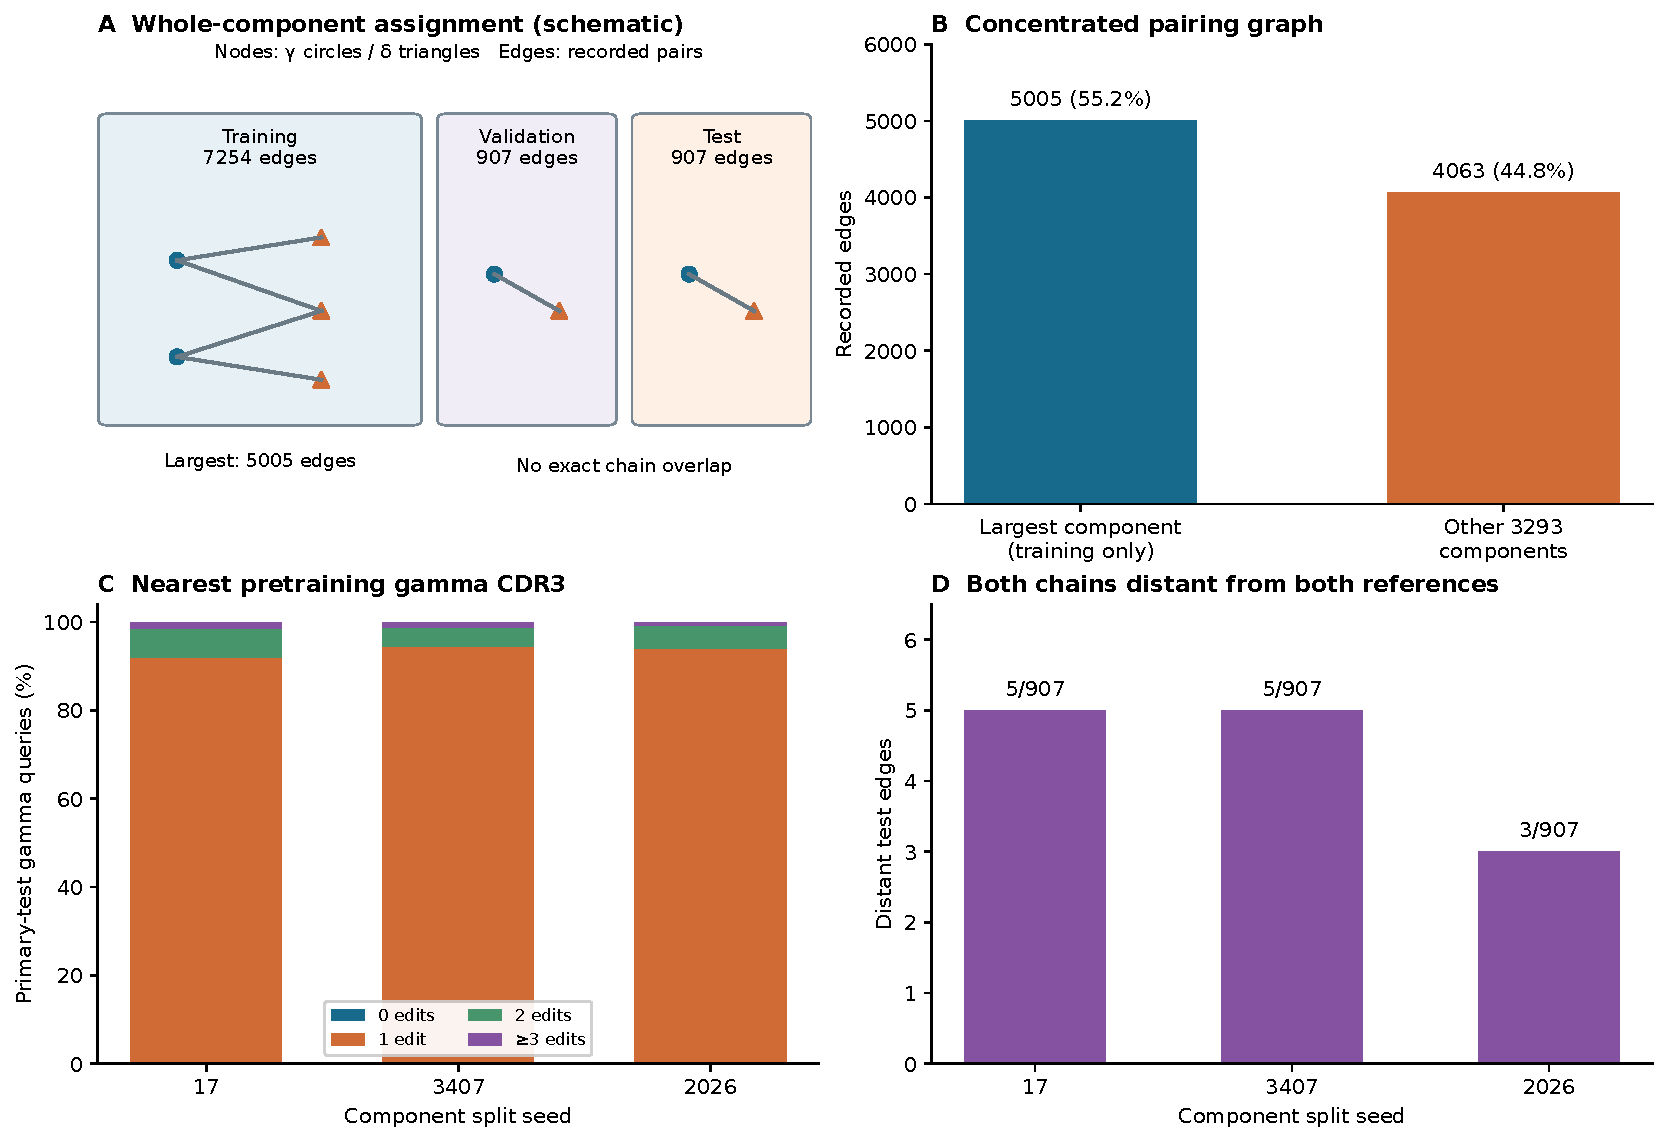
\includegraphics[width=\linewidth]{../results/bmc/figures/figure_2_data.pdf}
\caption{Pairing-graph concentration and sequence exposure. A: schematic component assignment, with all 5005 edges of the largest component retained in training. Nodes are unique gamma/delta CDR3s and edges are publicly recorded pairs. Primary partitions have no exact chain overlap. B: observed component concentration. C: minimum full-CDR3 Levenshtein distance to the pretraining pool. D: a distant edge requires both chains to be at least three edits from both supervised and pretraining references. The 5/5/3 distant-edge counts are too small for stable inferential transfer claims. This figure describes dataset exposure, not a recovery endpoint.}
\label{fig:data}
\end{figure}
\FloatBarrier

\subsection{Pretraining improves likelihood with a modest conditional contribution}
The conditional model achieves equal-direction query-macro NLL
$1.005\pm0.004$ nats per target token, compared with $1.013\pm0.003$ for
constant source, $1.115\pm0.006$ for random initialization and
$1.018\pm0.003$ for shuffled inputs (Table~\ref{tab:primary}).
These are means and descriptive SDs of three split means, each averaging two
model seeds. All six conditional-minus-prior NLL contrasts are negative,
approximately $-0.009$ to $-0.006$, with paired component-bootstrap intervals
below zero. Conditional-minus-random contrasts range from $-0.115$ to
$-0.104$ (Table~\ref{tab:paired}). The advantage over the matched prior
supports a modest contribution from the input under this training protocol.

The matched comparison is essential because the constant-source model shares
the denoising initialization and target sampling. Its strong likelihood can
therefore reflect a learned target distribution even after input residues are
removed. Shuffling additionally asks whether the fitted conditional model
benefits from the correct input association at evaluation. These controls
support interpretation of the NLL difference within the implemented training
scheme; they do not equate an average log-score improvement with a biological
pairing probability.

Frozen denoising evaluation also shows reconstruction beyond the aligned-copy
control: selected-residue accuracy is 71.3\%/70.3\% for gamma and
64.1\%/64.7\% for delta across seeds. These single-chain results support
reconstruction ability, while downstream matched controls establish the
likelihood comparison. Neither endpoint measures free partner recovery.
Pretraining-mixture and directional-training sensitivities are reported in
Additional file 1, Figure S1.

\begin{table}[!htbp]
\centering
\caption{Free generation at 64 draws with training targets allowed. Values are means and descriptive standard deviations of three split means, each averaging two model seeds. NLL is in nats per target token; coverage and Hit@5 are percentages. The equal mean weights directions equally. A dash denotes an unavailable scorer, not a zero outcome.}
\label{tab:primary}
\small
\setlength{\tabcolsep}{3pt}
\begin{tabular}{>{\raggedright\arraybackslash}p{0.2200\linewidth}p{0.1360\linewidth}p{0.1360\linewidth}p{0.1360\linewidth}p{0.1360\linewidth}p{0.1360\linewidth}}
\toprule
Model / direction & NLL & Coverage & Likelihood Hit@5 & Ranker Hit@5 & Fused Hit@5\\
\midrule
Conditional / \gtd{} & 1.253 $\pm$ 0.008 & 0.09 $\pm$ 0.16 & 0.00 $\pm$ 0.00 & 0.00 $\pm$ 0.00 & 0.00 $\pm$ 0.00\\
Conditional / \dtg{} & 0.757 $\pm$ 0.003 & 1.66 $\pm$ 0.23 & 0.06 $\pm$ 0.06 & 0.11 $\pm$ 0.06 & 0.06 $\pm$ 0.06\\
Conditional / Equal mean & 1.005 $\pm$ 0.004 & 0.88 $\pm$ 0.19 & 0.03 $\pm$ 0.03 & 0.06 $\pm$ 0.03 & 0.03 $\pm$ 0.03\\
Constant source / \gtd{} & 1.257 $\pm$ 0.007 & 0.00 $\pm$ 0.00 & 0.00 $\pm$ 0.00 & -- & --\\
Constant source / \dtg{} & 0.769 $\pm$ 0.003 & 1.00 $\pm$ 0.20 & 0.00 $\pm$ 0.00 & -- & --\\
Constant source / Equal mean & 1.013 $\pm$ 0.003 & 0.50 $\pm$ 0.10 & 0.00 $\pm$ 0.00 & -- & --\\
Random init. / \gtd{} & 1.377 $\pm$ 0.010 & 0.03 $\pm$ 0.05 & 0.00 $\pm$ 0.00 & 0.00 $\pm$ 0.00 & 0.00 $\pm$ 0.00\\
Random init. / \dtg{} & 0.853 $\pm$ 0.005 & 1.33 $\pm$ 0.22 & 0.00 $\pm$ 0.00 & 0.07 $\pm$ 0.03 & 0.02 $\pm$ 0.03\\
Random init. / Equal mean & 1.115 $\pm$ 0.006 & 0.68 $\pm$ 0.11 & 0.00 $\pm$ 0.00 & 0.04 $\pm$ 0.02 & 0.01 $\pm$ 0.02\\
Shuffled input / \gtd{} & 1.267 $\pm$ 0.006 & 0.03 $\pm$ 0.05 & 0.00 $\pm$ 0.00 & 0.00 $\pm$ 0.00 & 0.00 $\pm$ 0.00\\
Shuffled input / \dtg{} & 0.769 $\pm$ 0.001 & 1.33 $\pm$ 0.10 & 0.02 $\pm$ 0.03 & 0.15 $\pm$ 0.08 & 0.04 $\pm$ 0.03\\
Shuffled input / Equal mean & 1.018 $\pm$ 0.003 & 0.68 $\pm$ 0.07 & 0.01 $\pm$ 0.02 & 0.07 $\pm$ 0.04 & 0.02 $\pm$ 0.02\\
\bottomrule
\end{tabular}
\end{table}
\FloatBarrier

\subsection{Free recorded-partner recovery remains sparse}
At 64 draws, conditional coverage averages $0.88\pm0.19\%$ and likelihood
Hit@5 $0.03\pm0.03\%$. Constant source has $0.50\pm0.10\%$ coverage and no
top-five hits; random initialization has $0.68\pm0.11\%$ coverage and no
likelihood top-five hits. Conditional coverage is directional:
$0.09\pm0.16\%$ for \gtd{} and $1.66\pm0.23\%$ for \dtg{}
(Figure~\ref{fig:primary}). There are no \gtd{} top-five hits in any primary
conditional fit.

The conditional-minus-prior Hit@5 difference averages 0.03 percentage points.
The two event-bearing \dtg{} fits yield 2/900 versus 0/900 queries
(split 17, model seed 3407) and 1/906 versus 0/906 (split 3407, seed 3508).
All \gtd{} counts are zero in both conditions. After equal weighting of
directions, these differences are 0.11 percentage points
(95\% paired component-bootstrap interval $[0.00,0.27]$) and 0.06 points
($[0.00,0.17]$). The four remaining fits have zero difference and $[0,0]$
intervals (Table~\ref{tab:paired}). All six intervals include zero.
Overlapping splits and repeated fits are not pooled as independent biological
observations.

\begin{figure}[!htbp]
\centering
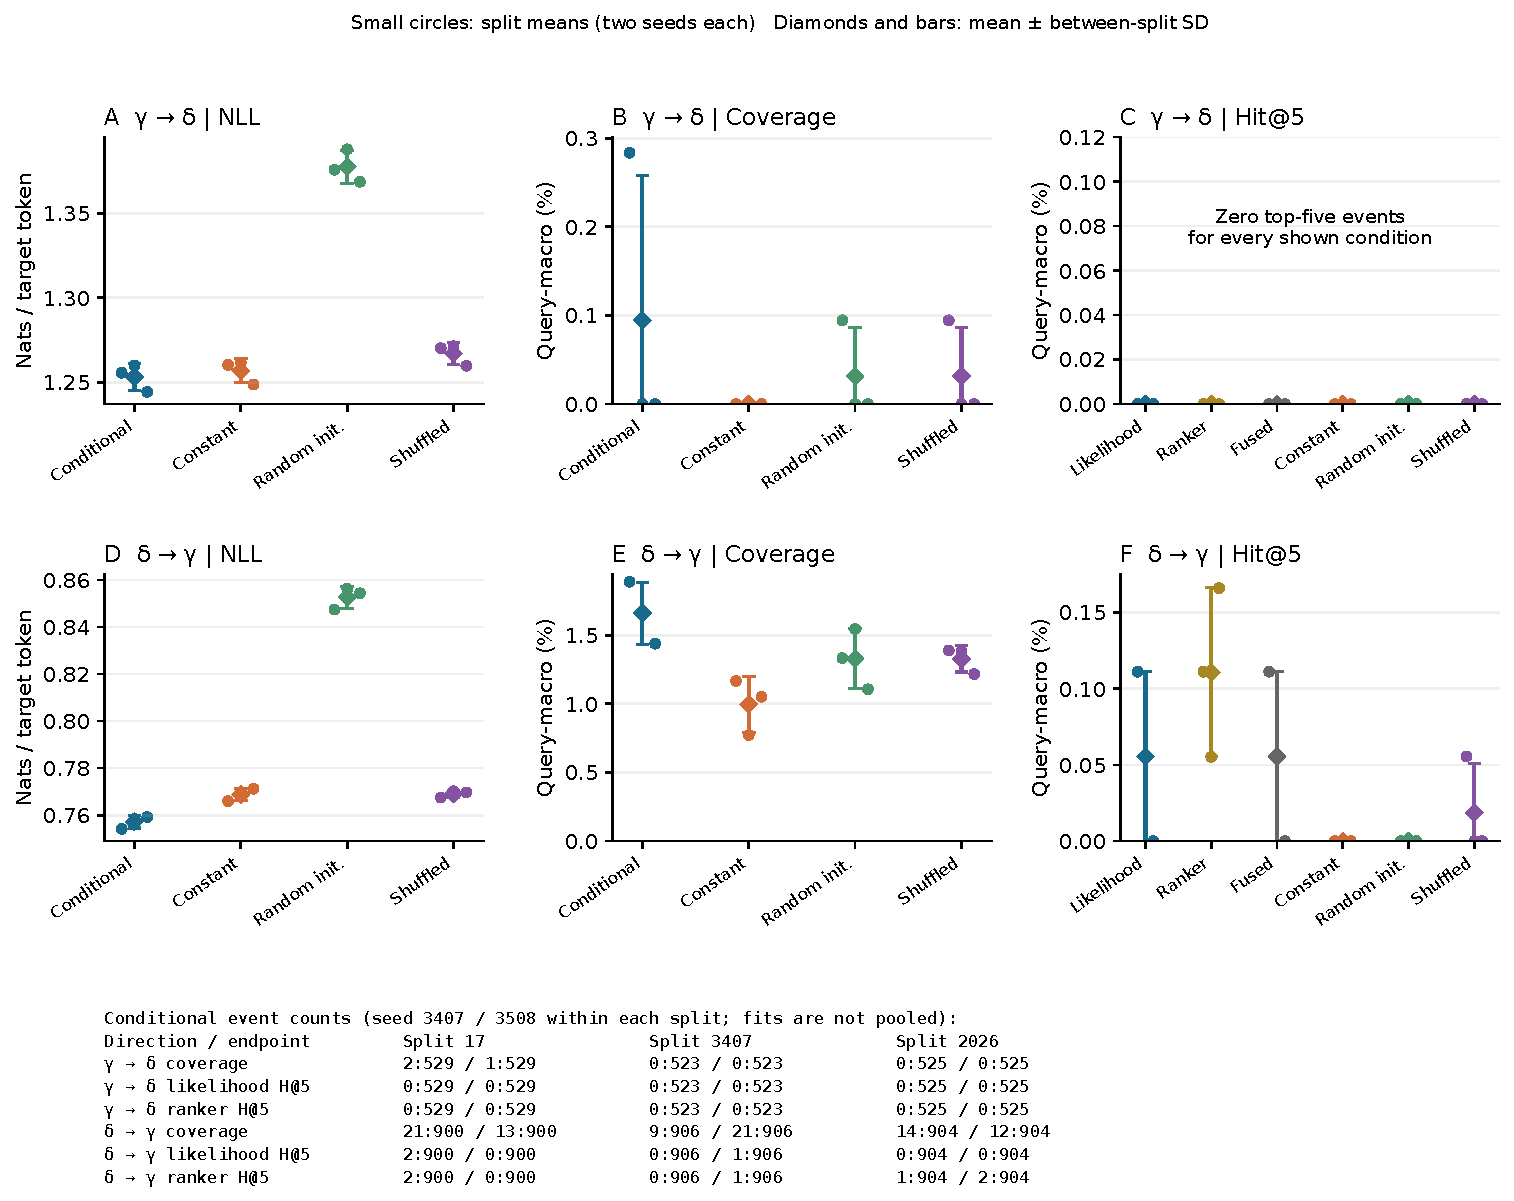
\includegraphics[width=\linewidth]{../results/bmc/figures/figure_3_primary.pdf}
\caption{Sparse free recorded-partner recovery at 64 draws. No recorded positive is injected into free candidates; training targets are allowed. Conditional, constant-source, random-initialization and shuffled-input conditions share the evaluation rule. Points are three split means after averaging two model seeds; diamonds and ranges are their mean and across-split descriptive SD, not confidence intervals. Likelihood, ranker and fused scores order identical conditional candidates. The graphic gives conditional events:query counts for each fitted model; all conditions are tabulated in Additional file 4. Zero events are retained. A lower NLL does not imply reliable candidate availability or top-five recovery.}
\label{fig:primary}
\end{figure}
\FloatBarrier

Ranker ordering gives equal-direction Hit@5 of $0.06\pm0.03\%$, but all six
paired ranker-minus-likelihood intervals include zero. Free-candidate tuning
selects zero ranker weight in every primary fit, making fused ordering
identical to likelihood. Alternative negative sampling also shows no
reproducible gain (Additional file 1, Figure S2).
The evidence for improved likelihood is consequently clearer than that for
improved primary recovery. Candidate scarcity constrains every ordering
method because a ranker cannot recover a partner absent from the candidate set.

Saved query outcomes show both failure stages. For split 17/model seed 3407
in the delta-to-gamma direction, 879 of 900 queries have no recorded partner
among the 64-draw candidates; 19 contain one outside the likelihood top five,
and two have a top-five hit. The corresponding gamma-to-delta counts are
527, two and zero among 529 queries. These descriptive counts illustrate why
better scoring alone has limited scope when most candidate sets contain no
recorded positive. Additional file 4 retains the corresponding identities,
events and denominators across every fitted primary comparison.

\begin{table}[!htbp]
\centering
\caption{Primary paired contrasts. The 95\% component-bootstrap percentile intervals condition on each fitted model pair and its saved samples. All endpoints are equal-direction query means at 64 draws. C denotes the pretrained conditional model and P the matched constant-source prior. NLL differences are nats per token; Hit@5 differences are percentage points. Negative NLL and positive Hit@5 differences favor the first named condition. Ranker and fusion contrasts reorder the conditional model's identical candidates. Intervals are not adjusted for multiple comparisons; a zero-event [0,0] interval is not a population upper bound.}
\label{tab:paired}
\small
\setlength{\tabcolsep}{3pt}
\par\smallskip\noindent\textbf{A: Generator contrasts}\par\smallskip
\begin{tabular}{@{}>{\raggedright\arraybackslash}p{0.23\linewidth}>{\raggedright\arraybackslash}p{0.23\linewidth}>{\raggedright\arraybackslash}p{0.23\linewidth}>{\raggedright\arraybackslash}p{0.23\linewidth}@{}}
\toprule
Split / model seed & NLL: C minus P & Hit@5: C minus P & NLL: C minus random\\
\midrule
17 / 3407 & \shortstack[l]{-0.007\\{}[-0.010, -0.004]} & \shortstack[l]{0.11\\{}[0.00, 0.27]} & \shortstack[l]{-0.109\\{}[-0.116, -0.102]}\\[3pt]
17 / 3508 & \shortstack[l]{-0.009\\{}[-0.012, -0.006]} & \shortstack[l]{0.00\\{}[0.00, 0.00]} & \shortstack[l]{-0.104\\{}[-0.111, -0.097]}\\[3pt]
3407 / 3407 & \shortstack[l]{-0.006\\{}[-0.009, -0.004]} & \shortstack[l]{0.00\\{}[0.00, 0.00]} & \shortstack[l]{-0.115\\{}[-0.123, -0.108]}\\[3pt]
3407 / 3508 & \shortstack[l]{-0.006\\{}[-0.009, -0.004]} & \shortstack[l]{0.06\\{}[0.00, 0.17]} & \shortstack[l]{-0.111\\{}[-0.118, -0.104]}\\[3pt]
2026 / 3407 & \shortstack[l]{-0.009\\{}[-0.011, -0.006]} & \shortstack[l]{0.00\\{}[0.00, 0.00]} & \shortstack[l]{-0.114\\{}[-0.121, -0.106]}\\[3pt]
2026 / 3508 & \shortstack[l]{-0.008\\{}[-0.010, -0.005]} & \shortstack[l]{0.00\\{}[0.00, 0.00]} & \shortstack[l]{-0.106\\{}[-0.113, -0.099]}\\[3pt]
\bottomrule
\end{tabular}
\par\smallskip\noindent\textbf{B: Ordering contrasts}\par\smallskip
\begin{tabular}{@{}>{\raggedright\arraybackslash}p{0.23\linewidth}>{\raggedright\arraybackslash}p{0.355\linewidth}>{\raggedright\arraybackslash}p{0.355\linewidth}@{}}
\toprule
Split / model seed & Hit@5: ranker minus likelihood & Hit@5: fused minus likelihood\\
\midrule
17 / 3407 & \shortstack[l]{0.00\\{}[-0.21, 0.22]} & \shortstack[l]{0.00\\{}[0.00, 0.00]}\\[3pt]
17 / 3508 & \shortstack[l]{0.00\\{}[0.00, 0.00]} & \shortstack[l]{0.00\\{}[0.00, 0.00]}\\[3pt]
3407 / 3407 & \shortstack[l]{0.00\\{}[0.00, 0.00]} & \shortstack[l]{0.00\\{}[0.00, 0.00]}\\[3pt]
3407 / 3508 & \shortstack[l]{0.00\\{}[-0.17, 0.16]} & \shortstack[l]{0.00\\{}[0.00, 0.00]}\\[3pt]
2026 / 3407 & \shortstack[l]{0.06\\{}[0.00, 0.17]} & \shortstack[l]{0.00\\{}[0.00, 0.00]}\\[3pt]
2026 / 3508 & \shortstack[l]{0.11\\{}[0.00, 0.28]} & \shortstack[l]{0.00\\{}[0.00, 0.00]}\\[3pt]
\bottomrule
\end{tabular}
\end{table}
\FloatBarrier

The sampling sensitivity reinforces the distinction between coverage and
top-five recovery. More draws increase \dtg{} coverage on split 17 without
ensuring higher Hit@5. Exact training-target exclusion changes ordering but
not primary coverage, and is evaluated separately from the primary policy.
Calibration has no recorded \gtd{} positives and only one to six \dtg{}
positive candidates per primary calibration set, limiting useful threshold
selection. Complete sampling, tuning and calibration results are in
Additional file 1, Figure S3.

\subsection{Diagnostic ranking in truth-containing candidate pools}
Fixed-pool retrieval is easier than free generation because the recorded
targets are supplied (Figure~\ref{fig:retrieval}). In random small pools,
conditional-likelihood Hit@5 averages 8.9\% for \gtd{} and 13.5\% for
\dtg{}, compared with 8.5\%/11.5\% for the prior and 8.0\%/5.1\% for seeded
random scores. Full-target retrieval gives 1.2\%/4.2\% for conditional
likelihood and 1.1\%/3.8\% for the prior. Fitted comparisons and their paired
uncertainty remain available in Additional file 4.

The conditional-minus-prior score depends strongly on direction and pool
construction. For \gtd{}, motif-pool Hit@5 rises from 5.4\% under
conditional likelihood to 12.4\%, while a shallow length/terminal-feature
model already reaches 11.8\%. For \dtg{}, the difference score reaches
6.0\% in motif pools and 1.0\% in full retrieval, below likelihood's
8.0\% and 4.2\%. Ranker values are 8.3\%/5.1\% in motif pools and
1.1\%/1.4\% in full retrieval. No scorer dominates all directions and pools.

The distractor rule changes which sequence features are useful for ordering.
A random small pool and a full target universe have different search spaces,
while motif- or edit-matched pools deliberately constrain similarity to the
positive. Their percentages consequently cannot be treated as interchangeable
estimates of unconstrained generation. In the primary chain-disjoint setting,
every training-target frequency score is zero, so its ordering is a
deterministic tie control. The benchmark retains that result rather than
interpreting it as informative frequency prediction.

Nearest-input partner-similarity ranking reaches random-pool Hit@5 of
9.2\%/7.9\% and full-pool Hit@5 of 1.5\% in both directions. It is
competitive with conditional likelihood in some \gtd{} pools, but does not
dominate \dtg{}. Direct transfer from either one or five nearest inputs has
zero primary hits because test targets are absent from training.
Its candidate restriction makes this zero structurally expected; it is
distinct from ranking supplied targets by partner similarity.
Neither outcome shows that a model has learned a biological pairing mechanism.

\begin{figure}[!htbp]
\centering
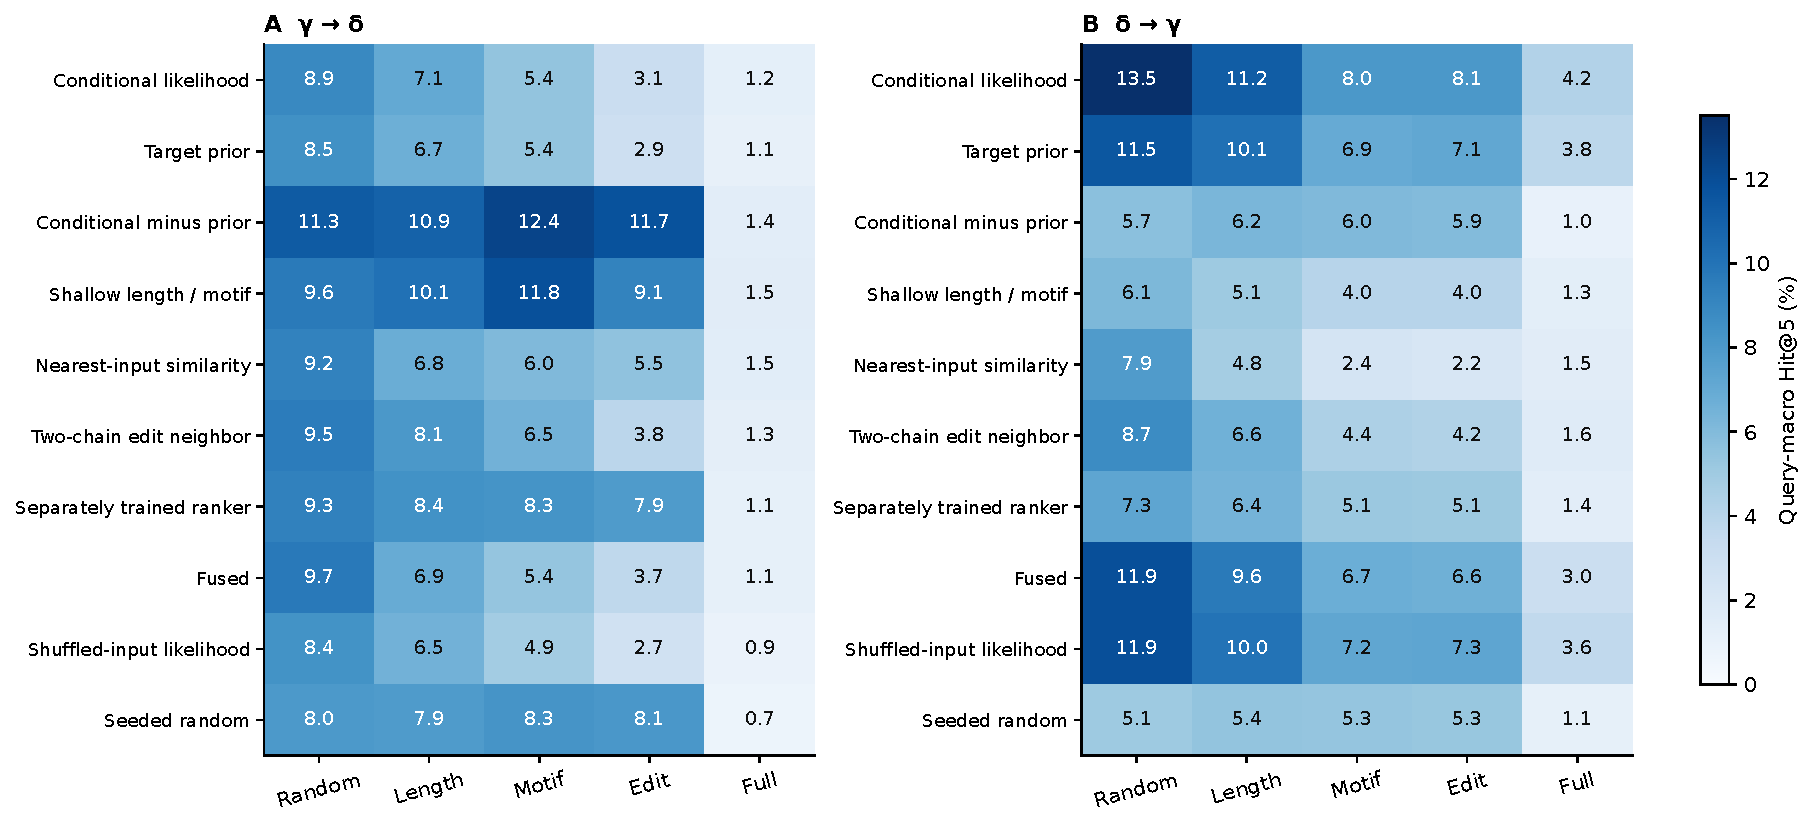
\includegraphics[width=\linewidth]{../results/bmc/figures/figure_4_retrieval.pdf}
\caption{Diagnostic ranking in truth-containing fixed candidate pools. Fixed pools contain recorded positives by construction. Random, length, motif and edit pools add up to 100 unrecorded distractors; Full uses the complete role-specific target universe. Values average seeds within split and then the three primary splits equally. Deterministic methods have one value per split. Nearest-input similarity scores candidates by target distance to partners of the single nearest training input; direct partner transfer is reported separately. No scorer dominates all pools and directions. These retrieval outcomes cannot be equated with free-generation recovery or biological specificity.}
\label{fig:retrieval}
\end{figure}
\FloatBarrier

\subsection{Training-size and graph-composition sensitivity}
Pretraining lowers NLL relative to random initialization at every actual
training size (Figure~\ref{fig:efficiency}). At 725 edges, two-seed pretrained
NLL is 1.273/0.780 for \gtd{}/\dtg{}, compared with 1.392/0.849 for random
initialization. At 2249 edges the values are 1.255/0.771 and 1.375/0.838;
at 7254 edges they are 1.256/0.754 and 1.376/0.847.
Random-model \dtg{} NLL is not monotonic in training size, and pretrained
\gtd{} NLL largely plateaus beyond 1814 edges.

The likelihood advantage does not produce a consistent small-data recovery
advantage. Across 725/1814/2249/7254 edges, pretrained \dtg{} likelihood
Hit@5 is 0.06/0.17/0.33/0.11\%, versus 0.22/0.44/0.17/0.00\% for random
initialization. Every \gtd{} likelihood Hit@5 remains zero.
The nominal 50\% subset contains only 31.0\% of training edges, because the
5005-edge component cannot be split. All smaller subsets contain only
singleton components, and the giant component enters at full data.
These curves describe joint sensitivity to training size and graph composition,
rather than pure sample complexity. Additional pretraining and negative
sampling analyses retain the same separation between likelihood and recovery
(Additional file 1).

\begin{figure}[!htbp]
\centering
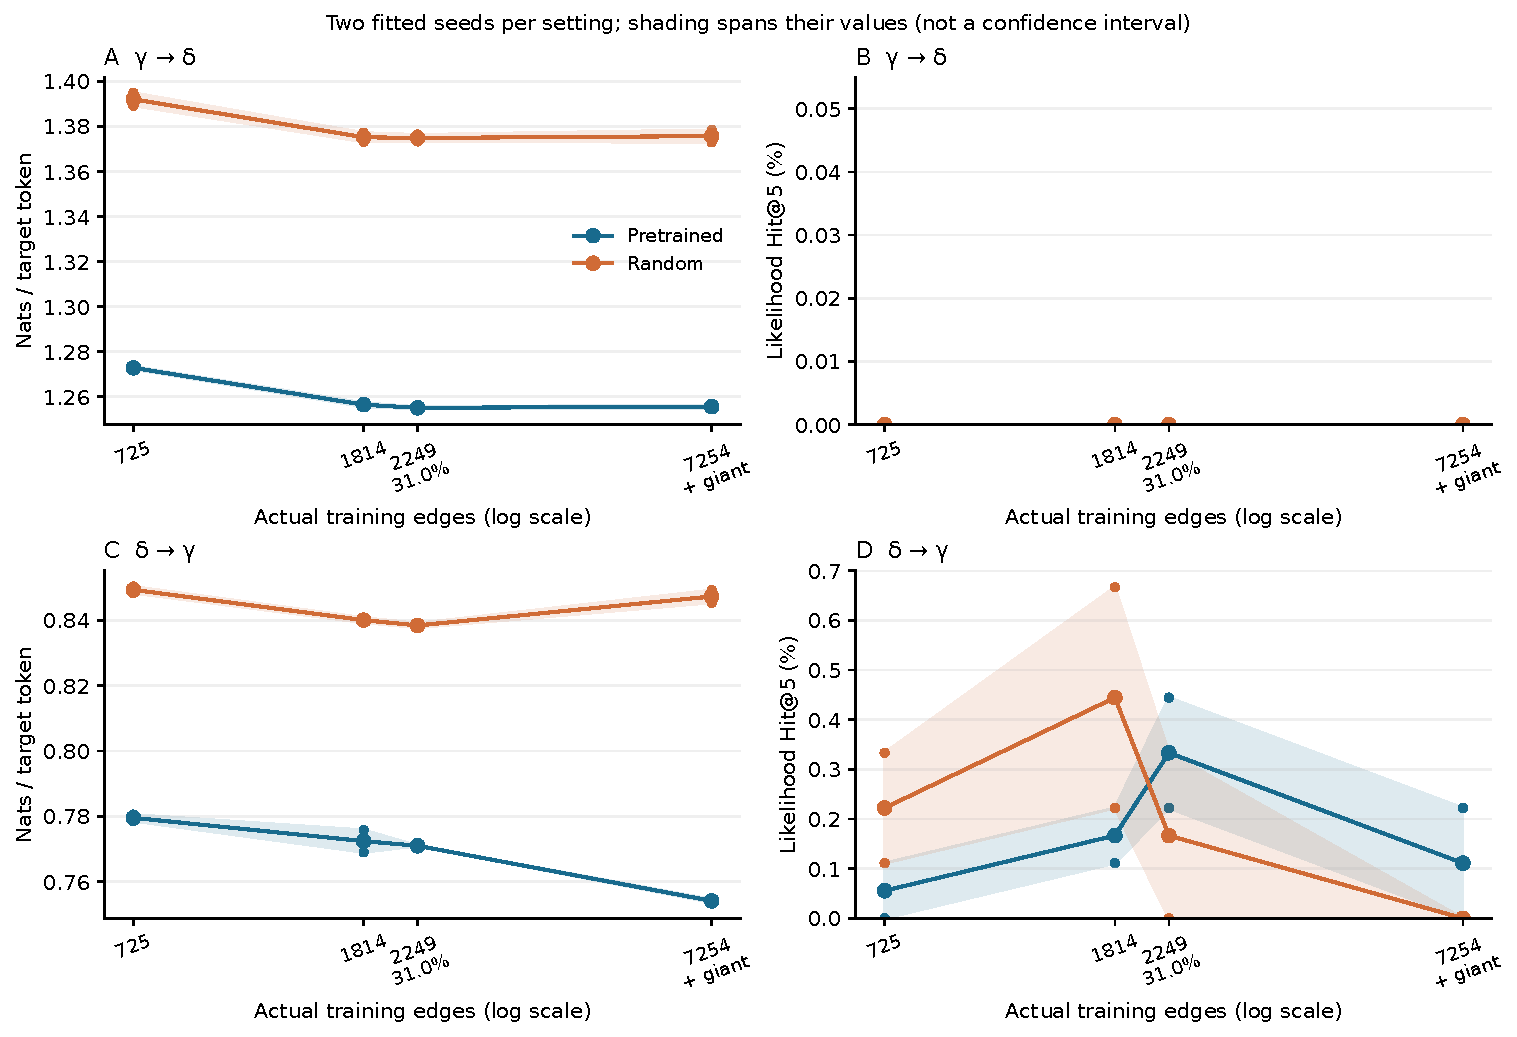
\includegraphics[width=\linewidth]{../results/bmc/figures/figure_5_efficiency.pdf}
\caption{Training-size and graph-composition sensitivity. The actual subsets contain 725/1814/2249/7254 edges. The nominal 50\% subset contains only 31.0\% of training edges. All smaller subsets contain singleton components; the giant component enters only at full data, so composition and size change together. Lines average two model seeds and shading spans their fitted estimates; it is not a confidence interval. Lower NLL does not provide a consistent small-data free-recovery advantage.}
\label{fig:efficiency}
\end{figure}
\FloatBarrier

\subsection{Recovery depends on exposure protocol}
Higher recovery appears in several exposed-target populations, but often with
strong prior or shuffled controls (Figure~\ref{fig:protocols}).
After unseen-gamma selection is reallocated across 31 queries with eligible
distractors, conditional likelihood recovers 8/64 and 10/64 test queries,
compared with 8/64 and 9/64 for constant source and 10/64 and 8/64 for random
initialization. Conditional-minus-prior differences are 0.00 percentage
points (95\% input-query interval $[0.00,0.00]$) and 1.56 points
($[0.00,4.69]$). Ranker ordering recovers 6/64 and 8/64.
These fits correct the original single-query selection problem, but the test
still permits target exposure and does not establish a reproducible
conditional advantage. Historical and complete per-control outcomes are
retained in Additional files 1 and 4.

Within the giant component, conditional likelihood recovers 60/177 and
50/177 gamma queries (33.90\%/28.25\%) and 123/261 and 118/261 delta
queries (47.13\%/45.21\%). Constant-source counts are 47/177 in both
gamma fits and 113/261 and 121/261 for delta; shuffled-input counts are
57/177 and 54/177, and 126/261 and 116/261, respectively.
Ranker ordering is worse than likelihood in all four fits.
All 500 test edges retain both endpoints in training and belong to one
original component. These counts therefore characterize withheld-edge
recovery within an exposed component, without an inferential
component-bootstrap interval or an unseen-component transfer claim.

\begin{figure}[!htbp]
\centering
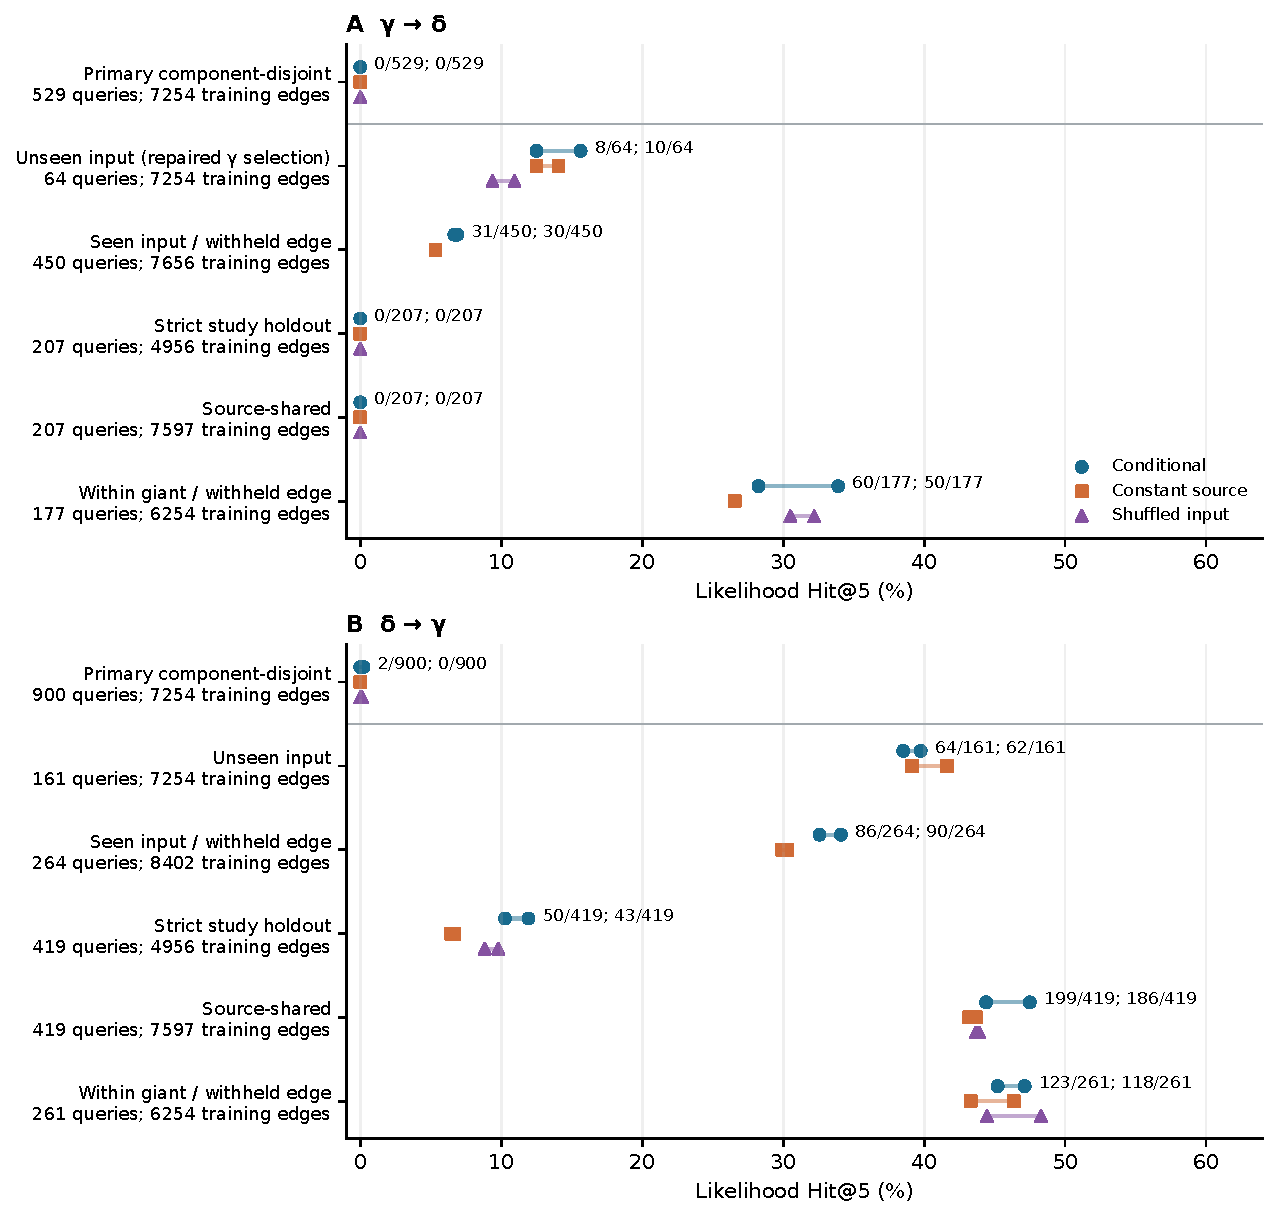
\includegraphics[width=\linewidth]{../results/bmc/figures/figure_6_protocols.pdf}
\caption{Recovery across distinct exposure populations. Each point is one model seed at 64 free draws; labels give conditional events/queries in seed order 3407;3508. The first row is the primary split-17 reference; all other rows are diagnostic populations with different training composition. Original unseen-gamma selection used a single query and had degenerate MRR; the plotted refits use 31 selection queries, leaving train/test membership unchanged. Unseen-input tasks permit target exposure; seen-input and within-giant tasks retain supervised input exposure, with both endpoints exposed in the latter. Missing shuffled points in original directional tasks mean not evaluated. Strict study holdout excludes held-study chains; source-shared retains common chains. Neither is donor-independent external validation. All within-giant edges arise from one original component; no inferential component interval is asserted.}
\label{fig:protocols}
\end{figure}
\FloatBarrier

For unseen delta inputs, conditional \dtg{} Hit@5 is 39.75\%/38.51\%,
versus 41.61\%/39.13\% for the prior. In seen-input tests it is
6.89\%/6.67\% for \gtd{} and 32.58\%/34.09\% for \dtg{}, versus
5.33\%/5.33\% and 30.30\%/29.92\% for the prior.
One seen-delta fitted contrast has a positive interval, but the two-seed
comparison is not uniform. The two seen-delta conditional-minus-prior
differences are 2.27 percentage points (95\% interval $[-1.52,6.06]$) and
4.17 points ($[0.38,8.33]$). The unseen-delta test has 161 queries and 244
distinct recorded target gammas shared with training. These populations and allowable overlaps differ
from the primary test; their detailed events and uncertainty remain separate.

Strict study holdout has 207 gamma and 419 delta queries over 626 pairs.
Conditional \dtg{} Hit@5 is 11.93\%/10.26\%, versus 6.68\%/6.44\% for
constant source. Conditional-minus-prior differences are 5.25 points
($[0.00,6.23]$) and 3.82 points ($[0.00,4.48]$), with both 95\% component
intervals reaching zero. Retaining shared supervised chains increases
conditional recovery to 47.49\%/44.39\%, while constant source reaches
43.68\%/43.20\%. Conditional \gtd{} Hit@5 is zero under both source
protocols, and ranker \dtg{} recovery remains below likelihood.

Source-task events are concentrated: the largest test component contains
529 of 626 edges and 323 of 419 delta queries, including 50 of 50 and 42
of 43 strict-source conditional hits. The source protocols share the test set
and filtered pretraining pool but use 4956 versus 7597 supervised training
edges. Recovery differences therefore combine exposure and training
composition. They support neither a donor-independent nor a distant-sequence
generalization claim. Complete contrasts, including positive fitted effects
and their limitations, are retained in Additional file 1.

\section{Discussion}
\subsection{Main findings}
This benchmark separates an improvement in sequence likelihood from reliable
recovery of a recorded paired chain. Denoising pretraining consistently
improves NLL over matched random initialization, and conditioning provides a
smaller advantage over the target prior. However, these improvements coexist
with sparse primary free-generation hits. The central limitation is often
candidate availability: even a successful ranking method cannot recover a
recorded positive that the generator did not sample. The separately trained
ranker supplies no reproducible primary benefit, and tuning favors likelihood
alone for free candidates.

These findings qualify the interpretation of generative performance without
negating the observed likelihood advantage. Pretraining and conditioning can
improve the distribution assigned to targets while leaving recovery at a
specified finite budget too low for practical partner selection.
The result is consistent with treating representation learning, conditional
modeling and sequence recovery as separate empirical questions, as motivated
by prior work on downstream pretraining effects \cite{landry2025}.
It does not imply that every architecture or decoding strategy must fail.

\subsection{Sequence neighborhoods and exposure}
Sequence and graph exposure explain why the evaluation populations require
separate interpretation. The primary test excludes exact training chains,
yet most test gamma queries remain one edit from the pretraining pool.
The largest pairing component is restricted to training, and the distant
test subset is too small for a stable estimate. Thus, exact-chain separation
defines a useful benchmark boundary but does not establish transfer to a
diverse population of remote sequences.

Nearest-input partner-similarity ranking demonstrates that local neighborhoods
can be informative in a constructed retrieval task. It scores a supplied
withheld target through similarity to known training partners without
proposing that target. Direct transfer can only return training targets and
is structurally zero when exact test targets are excluded.
Its failure cannot establish the learned model's superiority over
sequence-neighborhood information. Neither comparison proves memorization
of training pairs or identifies a biological mechanism. Target priors,
near-neighbor pretraining exposure and simple sequence regularities remain
possible contributors that the current controls do not fully disentangle.
A paired-domain retrieval preprint also reports that reducing neighbor
hubness does not guarantee improved specificity retrieval \cite{hubness}.
That study concerns different receptors and representations; it does not
identify the failure mechanism of the present generator.

Higher recovery in source and target-exposed tasks is also a substantive
result, including positive fitted conditional-minus-prior differences under
strict source holdout. Strong prior and shuffled baselines, clustered events
and changing supervised composition limit attribution to conditional
information. Differences in chain distributions and partner multiplicity
could contribute to directional asymmetry, but the experiments do not isolate
their biological causes.

\subsection{Implications for evaluation design}
Evaluation should report likelihood, candidate coverage and ranking success
as distinct endpoints. A fixed pool that contains recorded positives provides
a controlled ordering comparison, while free generation additionally tests
whether those sequences are produced. Likewise, training-target exclusion
has different consequences when test targets are unseen and when valid
positives are exposed. Reporting only the most favorable protocol would
obscure these differences.

Matched priors and neighborhood controls help identify what an apparent
improvement actually requires. Pairing graphs should inform both partitions
and uncertainty: one giant component cannot provide independent component
replicates, and overlapping graph splits or repeated seeds do not create
independent biological observations. Validation roles also need adequate
query groups and ranking distractors. The unseen-gamma sensitivity illustrates
why an edge-count allocation can leave checkpoint selection uninformative
even when the nominal validation set is large.

The uncertainty statements are similarly tied to their sampling units.
Component-bootstrap intervals describe test-query variation conditional on
the fitted models and saved samples, whereas the across-split SD describes
variation between the three split means. Neither measures all uncertainty
from future cohort sampling, optimization choices or hardware variation.
In particular, an empirical zero-event interval does not exclude rare recovery
in a larger population. Reporting counts alongside percentages makes this
limitation visible when the primary signal consists of only a few queries.

\subsection{Limitations and future work}
The paired corpus is small relative to unpaired sequence collections and is
dominated by developmental-thymic data. Recorded labels are incomplete, CDR3
boundary conventions differ across sources, and comparable cell-quality and
donor information are unavailable for some exports. One IEDB pair lacks
resolved original-study provenance. These limitations constrain the
population represented by the benchmark and the meaning of an unrecorded
combination. Recorded recovery does not establish receptor expression,
antigen recognition or functional compatibility.

The tested architecture and training budgets cover only one model family.
Random initialization matches downstream optimization but does not receive
equivalent total computation or separate tuning to establish its best
attainable performance. The frozen decoding rule estimates performance at a
specified budget, not each condition's optimum. Source comparisons and nested
training subsets also alter composition along with exposure or size.
The current results therefore do not establish general pretraining efficiency,
an optimal data requirement or intrinsic non-identifiability.

A stronger external evaluation would require a newly frozen cohort with
traceable donor/library metadata and sufficient distant gamma/delta pairs.
Training-size studies should separate composition from count, and
initialization comparisons should add validation tuning and matched total
computation. Functional claims would require independent experimental
evidence. Those extensions would address specific limitations while retaining
separate sequence-recovery, retrieval and functional endpoints.

\section{Conclusions}
Denoising pretraining improves target-token likelihood, with a modest
conditional contribution beyond a matched target prior. Free recorded-partner
recovery remains sparse under component-disjoint evaluation, and separate
ranking shows no reproducible primary benefit. Exposure and graph composition
limit broader transfer claims. Gamma-delta TCR partner benchmarks should
therefore report sequence modeling, candidate availability, recovery and
exposure dependence as separate outcomes.

\section*{Abbreviations}
CDR3: complementarity-determining region 3; TCR: T-cell receptor;
NLL: negative log likelihood; EOS: end of sequence;
MRR: mean reciprocal rank; SD: standard deviation;
GEO: Gene Expression Omnibus; IEDB: Immune Epitope Database;
GPU: graphics processing unit; AUC: area under the curve;
HLA: human leukocyte antigen; MHC: major histocompatibility complex.

\section*{Availability of data and code}
Original input exports, cleaned sequences, provenance, frozen partitions,
source snapshots and reference results are available at
\url{https://github.com/he2238751697-afk/GDTCR}, scientific release
\texttt{reproducibility-v1} (commit
\texttt{fcf153c76d8eeac358d1a26da3df470eb4118992}).
The input exports are processed sequence/contig/database files rather than raw
FASTQ reads. Upstream accessions include GSE180059 and E-MTAB-11388;
source-specific access and terms are documented in
\texttt{THIRD\_PARTY\_DATA.md}. The repository provides reconstruction and
execution instructions in \texttt{REPRODUCIBILITY.md}, with a separately
distributed initialization asset verified by checksum. Third-party materials
retain their source-specific terms.

\section*{Supplementary materials}
Additional file 1 contains supplementary methods, sensitivity analyses and
Figures S1--S3. Additional file 2 provides dataset, source, graph and distance
audits. Additional file 3 records seeds, checkpoint identifiers, run settings
and training exposure. Additional file 4 contains primary and diagnostic
query outcomes, event counts and paired contrasts. Additional file 5 provides
split assignments, fixed candidate pools and free-candidate hashes.
Additional file 6 contains source, frozen configurations, environments and
reproduction instructions.

\begin{thebibliography}{99}
\bibitem{gd_review} Adams EJ, Gu S, Luoma AM.
Human gamma delta T cells: Evolution and ligand recognition.
Cellular Immunology. 2015;296(1):31--40. doi:10.1016/j.cellimm.2015.04.008.
\bibitem{uctcrdb} Dou Y, Shan S, Zhang J.
UcTCRdb: An unconventional T cell receptor sequence database with online analysis
functions. Frontiers in Immunology. 2023;14:1158295.
doi:10.3389/fimmu.2023.1158295.
\bibitem{tcrdb2} Yue T, Chen SY, Shen WK, et al.
TCRdb 2.0: an updated T-cell receptor sequence database.
Nucleic Acids Research. 2026;54(D1):D504--D510.
doi:10.1093/nar/gkaf876.
\bibitem{ots} Raybould MIJ, Greenshields-Watson A, Agarwal P, et al.
The Observed T Cell Receptor Space database enables paired-chain repertoire
mining, coherence analysis, and language modeling.
Cell Reports. 2024;43(9):114704. doi:10.1016/j.celrep.2024.114704.
\bibitem{tcrbert} Wu K, Yost KE, Daniel B, et al.
TCR-BERT: learning the grammar of T-cell receptors for flexible antigen-binding
analyses. bioRxiv [preprint]. 2021. doi:10.1101/2021.11.18.469186.
\bibitem{tcrbinder} Dong W, Yang Q, Xu L, et al.
TCRBinder: Unified pre-trained language model with paired-chain synergy for
predicting T-cell receptor binding specificity.
PLoS Computational Biology. 2026;22(6):e1014396. doi:10.1371/journal.pcbi.1014396.
\bibitem{tcrdesign} Li X, Yang Q, Xu L, et al.
TCRdesign: an antigen-specific generative language model for de novo design of
T-cell receptors. Briefings in Bioinformatics. 2025;26(6):bbaf691.
doi:10.1093/bib/bbaf691.
\bibitem{landry2025} Landry B, Zhang J.
Masked language modeling pretraining dynamics for downstream peptide:
T-cell receptor binding prediction. Bioinformatics Advances. 2025;5(1):vbaf028.
doi:10.1093/bioadv/vbaf028.
\bibitem{pairing_constraints} Milighetti M, Nagano Y, Henderson J, et al.
Systematic analysis of CDR contacts and pairing constraints between T cell
receptor alpha/beta chains.
Bioinformatics. 2026;42(8):btag551. doi:10.1093/bioinformatics/btag551.
\bibitem{tcrpair} M\"osch A, Frishman D.
TCRpair: prediction of functional pairing between HLA-A*02:01-restricted
T-cell receptor alpha and beta chains.
Bioinformatics. 2021;37(21):3938--3940. doi:10.1093/bioinformatics/btab573.
\bibitem{dtcr} Wang H, Zang T, Liu Y.
DTCR: generating realistic, diverse, and epitope-specific T cell receptor
sequences via a discrete diffusion model. Briefings in Bioinformatics.
2026;27(4):bbag438. doi:10.1093/bib/bbag438.
\bibitem{germline_shortcut} Wang S, Sengupta A, Li S, Standley DM.
A germline shortcut in protein language model retrieval of adaptive immune
receptors. bioRxiv [preprint]. 2026. doi:10.64898/2026.07.21.739963.
\bibitem{af3_specificity} Woods LJ, Neff B, Lahouel K, et al.
General prediction of T cell receptor antigen specificity from sequence using AlphaFold 3.
Science Advances. 2026;12(44):eaef5674. doi:10.1126/sciadv.aef5674.
\bibitem{gse180059} Sanchez Sanchez G, Papadopoulou M, Azouz A, et al.
Identification of distinct functional thymic programming of fetal and pediatric
human gamma-delta thymocytes via single-cell analysis.
Nature Communications. 2022;13(1):5842. doi:10.1038/s41467-022-33488-2.
\bibitem{suo2022} Suo C, Dann E, Goh I, et al.
Mapping the developing human immune system across organs.
Science. 2022;376(6597):eabo0510. doi:10.1126/science.abo0510.
\bibitem{iedb} Vita R, Blazeska N, Marrama D, et al.
The Immune Epitope Database (IEDB): 2024 update.
Nucleic Acids Research. 2025;53(D1):D436--D443. doi:10.1093/nar/gkae1092.
\bibitem{pr_metrics} Saito T, Rehmsmeier M.
The precision-recall plot is more informative than the ROC plot when evaluating
binary classifiers on imbalanced datasets.
PLoS ONE. 2015;10(3):e0118432. doi:10.1371/journal.pone.0118432.
\bibitem{hubness} Maire K, Zheng W.
Hubness and local scaling in paired T cell receptor distance spaces.
bioRxiv [preprint]. 2026. doi:10.64898/2026.10.13.758726.
\end{thebibliography}
\end{document}
